\documentclass{article}
\usepackage{amsmath, amssymb, amsthm, pgfplots}
\pgfplotsset{compat=1.8}

% Definir estilos
\theoremstyle{definition} 
\newtheorem{problem}{Problema} 
\newtheorem*{solution}{Solución} 

\begin{document}

\title{Ejercicios del Apartado 2.2. (p. 57)}
\author{Simmons, George F. \\ \textit{Calculus with Analytic Geometry. 2nd ed.}}
\date{Febrero de 2025}
\maketitle

\begin{problem} 
Encuentra la ecuación de la recta tangente a la parábola \( y = x^2 \).
\begin{enumerate}
    \item En el punto \((-2,4)\).
    \item En el punto donde la pendiente es \(8\).
    \item Si la intersección con el eje \( x \) de la tangente es \(2\).
\end{enumerate}
\end{problem}

\begin{solution}
Sea \( f(x)=x^2 \) con derivada \( f'(x)=2x \).

\medskip

\textbf{Inciso 1:} En el punto \((-2,4)\).\\
Se tiene \( x_0=-2 \) y
\[
f'(-2)=2(-2)=-4
\]
La ecuación de la recta tangente es:
\begin{align*}
y-4 &= -4\bigl(x-(-2)\bigr)\\
y-4 &= -4\,(x+2)\\
y &= -4x - 8 + 4\\
y &= -4x - 4
\end{align*}

\textbf{Inciso 2:} En el punto donde la pendiente es \(8\).\\
Igualamos la derivada a \(8\):
\[
2x_0=8 \quad\Longrightarrow\quad x_0=4.
\]
Luego, \( y_0=f(4)=4^2=16 \). La recta tangente es:
\begin{align*}
y-16 &= 8\,(x-4)\\
y-16 &= 8x-32\\
y &= 8x - 16.
\end{align*}

\textbf{Inciso 3:} La tangente pasa por \((2,0)\).\\
Sea el punto de tangencia \((a, a^2)\). La recta tangente general es:
\[
y=2a\,(x-a)+a^2.
\]
La condición de que pase por \((2,0)\) es:
\begin{align*}
0 &= 2a\,(2-a)+a^2\\
0 &= 4a - 2a^2 + a^2\\
0 &= 4a - a^2\\
a^2-4a &= 0\\
a(a-4)&=0.
\end{align*}
Se obtiene \( a=0 \) o \( a=4 \). La tangente para \( a=0 \) es \( y=0 \) (el eje \( x \)); por lo tanto, la otra tangente corresponde a \( a=4 \):
\[
y=2(4)\,(x-4)+4^2=8\,(x-4)+16=8x-32+16=8x-16.
\]
\end{solution}

\bigskip

\begin{problem}
Demuestra que la tangente a la parábola \( y = x^2 \) en un punto \((x_0,y_0)\), distinto del vértice, siempre tiene una intersección con el eje \( x \) en \(\frac{1}{2}x_0\).
\end{problem}

\begin{solution}
La ecuación de la recta tangente en \((x_0,x_0^2)\) es:
\[
y-x_0^2=2x_0\,(x-x_0).
\]
Para hallar la intersección con el eje \( x \), ponemos \( y=0 \):
\begin{align*}
0 - x_0^2 &= 2x_0\,(x-x_0)\\
-x_0^2 &= 2x_0\,x - 2x_0^2\\
x_0^2 &= 2x_0\,x\\
x &= \frac{x_0^2}{2x_0} = \frac{x_0}{2}.
\end{align*}
\end{solution}

\bigskip

\begin{problem}
Una recta de la forma \( y = mx + b \) es presumiblemente su propia tangente en cualquier punto. Verifica esto utilizando la fórmula del cociente diferencial para demostrar que si \( f(x) = mx + b \) entonces \( f'(x_0) = m \).
\end{problem}

\begin{solution}
Recordemos que:
\[
f'(x_0)=\lim_{\Delta x\to 0}\frac{f(x_0+\Delta x)-f(x_0)}{\Delta x}.
\]
Con \( f(x)=mx+b \) se tiene:
\[
f(x_0+\Delta x)=m(x_0+\Delta x)+b = mx_0 + m\Delta x + b,
\]
y
\[
f(x_0)=mx_0+b.
\]
Luego,
\[
f'(x_0)=\lim_{\Delta x\to 0}\frac{mx_0+m\Delta x+b-(mx_0+b)}{\Delta x}=\lim_{\Delta x\to 0}\frac{m\Delta x}{\Delta x}=m.
\]
\end{solution}

\bigskip

\begin{problem}
Dibuja el gráfico de la función \( y = x - x^2 \) en el intervalo \( -2 \leq x \leq 3 \).
\begin{enumerate}
    \item Usa el método de incrementos para calcular la pendiente de la recta tangente en un punto arbitrario \((x_0, y_0)\) de la curva.
    \item ¿Cuáles son las pendientes de las rectas tangentes en los puntos \((-1,-2)\), \((0,0)\), \((1,0)\) y \((2,-2)\)? Usa estas pendientes para dibujar las tangentes en estos puntos en tu gráfico.
    \item ¿En qué punto de la curva la tangente es horizontal?
\end{enumerate}
\end{problem}

\begin{solution}
Sea \( f(x)=x-x^2 \).

\medskip

\begin{center}
    \begin{tikzpicture}
        \begin{axis}[
            axis lines = middle, % Ejes en el centro
            xlabel = \( x \),
            ylabel = \( y \),
            samples = 100, % Suaviza la curva
            domain=-2:3, % Intervalo de x
            axis equal  % Mantiene la proporción real de los ejes
        ]
            
        % Dibuja la función y = x - x^2
        \addplot[blue, thick] {x - x^2};
    
        % Tangente en (-1,-2)
        \addplot[red, dashed, thick] {-3*(x + 1) - 2};
    
        % Tangente en (0,0)
        \addplot[green, dashed, thick] {1*(x - 0)};
    
        % Tangente en (1,0)
        \addplot[orange, dashed, thick] {-1*(x - 1)};
    
        % Tangente en (2,-2)
        \addplot[purple, dashed, thick] {-3*(x - 2) - 2};
    
        \end{axis}
    \end{tikzpicture}
\end{center}

\textbf{Inciso 1:}
Para un incremento \( h \), tenemos:
\[
f(x_0+h)=(x_0+h)-(x_0+h)^2.
\]
Expandiendo:
\[
(x_0+h)^2=x_0^2+2x_0h+h^2,
\]
se obtiene:
\[
f(x_0+h)=x_0+h-x_0^2-2x_0h-h^2.
\]
La variación en \( y \) es:
\[
\Delta y=f(x_0+h)-f(x_0)=h-2x_0h-h^2.
\]
Dividiendo por \( h \):
\[
\frac{\Delta y}{h}=1-2x_0-h.
\]
Tomando el límite \( h\to 0 \), se concluye que:
\[
f'(x_0)=1-2x_0.
\]

\textbf{Inciso 2:}
\begin{itemize}
    \item En \((-1,-2)\):
    \[
    f'(-1)=1-2(-1)=3.
    \]
    \item En \((0,0)\):
    \[
    f'(0)=1-2(0)=1.
    \]
    \item En \((1,0)\):
    \[
    f'(1)=1-2(1)=-1.
    \]
    \item En \((2,-2)\):
    \[
    f'(2)=1-2(2)=-3.
    \]
\end{itemize}

\textbf{Inciso 3:}\\
La recta tangente es horizontal cuando \( f'(x_0)=0 \):
\[
1-2x_0=0 \quad\Longrightarrow\quad x_0=\frac{1}{2}.
\]
\end{solution}

\bigskip

\begin{problem}
Usa la fórmula del cociente diferencial para calcular \( f'(x_0) \) si \( f(x) \) es:
\begin{enumerate}
    \item \( x^2 - 4x - 5 \).
    \item \( x^2 - 2x + 1 \).
    \item \( 2x^2 + 1 \).
    \item \( x^2 - 4 \).
\end{enumerate}
Los resultados serán necesarios en los problemas 6--9.
\end{problem}

\begin{solution}
\textbf{Inciso 1}

Calculamos \( f(x_0+\Delta x)-f(x_0)\) para \( x^2 - 4x - 5 \):

    \begin{align*}
    f(x_0+\Delta x)-f(x_0) &= [(x_0+\Delta x)^2-4(x_0+\Delta x)-5]-[x_0^2-4x_0-5] \\
    &= x_0^2 + 2x_0\Delta x + \Delta x^2 - 4x_0 - 4\Delta x - 5 + x_0^2 + 4x_0 + 5 \\
    &= 2x_0\Delta x + \Delta x^2 - 4 \Delta x
    \end{align*}

Divididmos el resultado por \( \Delta x \):

    \begin{align*}
    &= \frac{2x_0\Delta x + \Delta x^2 - 4 \Delta x}{\Delta x} \\
    &= 2x_0 + \Delta x - 4
    \end{align*}

Calculamos el límite para \( \Delta x \to 0 \):

    \begin{align*}
        &= \lim_{\Delta x \to 0} 2x_0 + \Delta x - 4 \\
        &= 2x_0 - 4
    \end{align*}

\textbf{Inciso 2}

Calculamos \( f(x_0+\Delta x)-f(x_0)\) para \( x^2 - 2x + 1 \):

    \begin{align*}
    f(x_0+\Delta x)-f(x_0) &= [(x_0+\Delta x)^2-2(x_0+\Delta x)+1]-[x_0^2-2x_0+1] \\
    &= x_0^2 + 2x_0\Delta x + \Delta x^2 - 2x_0 - 2\Delta x + 1 + x_0^2 + 2x_0 - 1 \\
    &= 2x_0\Delta x + \Delta x^2 - 2 \Delta x
    \end{align*}

Divididmos el resultado por \( \Delta x \):

    \begin{align*}
    &= \frac{2x_0\Delta x + \Delta x^2 - 2 \Delta x}{\Delta x} \\
    &= 2x_0 + \Delta x - 2
    \end{align*}

Calculamos el límite para \( \Delta x \to 0 \):

    \begin{align*}
        &= \lim_{\Delta x \to 0} 2x_0 + \Delta x - 2 \\
        &= 2x_0 - 2
    \end{align*}

\textbf{Inciso 3}

Calculamos \( f(x_0+\Delta x)-f(x_0)\) para \( 2x^2 + 1 \):

    \begin{align*}
    f(x_0+\Delta x)-f(x_0) &= [2(x_0+\Delta x)^2+1]-[2x_0^2+1] \\
    &= 2(x_0^2 + 2x_0\Delta x + \Delta x^2) +1 - 2x_0^2 - 1 \\
    &= 2x_0^2 + 4x_0 \Delta x + 2 \Delta x^2 + 1 - 2x_0^2 - 1 \\
    &= 4x_0 \Delta x + 2 \Delta x^2
    \end{align*}

Divididmos el resultado por \( \Delta x \):

    \begin{align*}
    &= \frac{4x_0 \Delta x + 2 \Delta x^2}{\Delta x} \\
    &= 4x_0 + 2\Delta x
    \end{align*}

Calculamos el límite para \( \Delta x \to 0 \):

    \begin{align*}
        &= \lim_{\Delta x \to 0} 4x_0 + 2\Delta x \\
        &= 4x_0
    \end{align*}

\textbf{Inciso 4}

Calculamos \( f(x_0+\Delta x)-f(x_0)\) para \( x^2 -4 \):

    \begin{align*}
    f(x_0+\Delta x)-f(x_0) &= [(x_0+\Delta x)^2-4]-[x_0^2-4] \\
    &= x_0^2 + 2x_0\Delta x + \Delta x^2 -4 - x_0^2 + 4 \\
    &= 2x_0 \Delta x + \Delta x^2
    \end{align*}

Divididmos el resultado por \( \Delta x \):

    \begin{align*}
    &= \frac{2x_0 \Delta x + \Delta x^2}{\Delta x} \\
    &= 2x_0 + \Delta x
    \end{align*}

Calculamos el límite para \( \Delta x \to 0 \):

    \begin{align*}
        &= \lim_{\Delta x \to 0} 2x_0 + \Delta x \\
        &= 2x_0
    \end{align*}
\end{solution}

\bigskip

\begin{problem}
Dibuja la curva y la recta tangente en el punto indicado, y encuentra la ecuación de esta recta tangente:
\begin{enumerate}
    \item \( y = x^2 - 4x - 5 \), en \((4,-5)\).
    \item \( y = x^2 - 2x + 1 \), en \((-1,4)\).
\end{enumerate}
\end{problem}

\begin{solution}
\textbf{Inciso 1:} Graficamos \( y = x^2 - 4x - 5 \): 

\begin{center}
    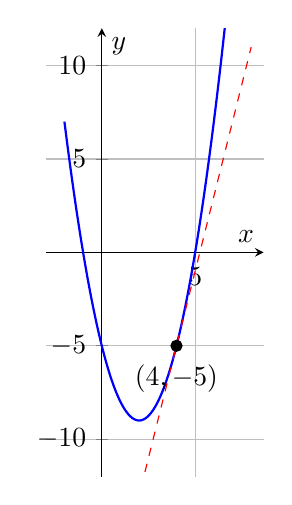
\begin{tikzpicture}
        \begin{axis}[
            axis lines = middle,
            xlabel = $x$,
            ylabel = $y$,
            grid = major,
            samples = 100,
            enlargelimits = true,
            domain = -2:8,
            ymin = -10, ymax = 10, % Ajustar el rango para mejor visualización
            axis equal image, % Mantiene la proporcionalidad entre ejes
        ]
            % Graficar la parábola
            \addplot[blue, thick] {x^2 - 4*x - 5};
    
            % Graficar la recta tangente
            \addplot[red, dashed] {4*(x-4) - 5};
    
            % Punto (4, -5)
            \addplot[only marks, mark=*, black] coordinates {(4,-5)};
            \node at (axis cs:4,-5.5) [anchor=north] {$(4, -5)$};
        \end{axis}
    \end{tikzpicture}
\end{center}

La derivada es:
\[
f'(x)=2x-4.
\]
En \( x=4 \):
\[
f'(4)=2(4)-4=4.
\]
La ecuación de la tangente es:
\begin{align*}
y-(-5) &= 4(x-4)\\
y+5 &= 4x-16\\
y &= 4x-21.
\end{align*}

\textbf{Inciso 2:} Graficamos \( y = x^2 - 2x + 1 \): 

\begin{center}
    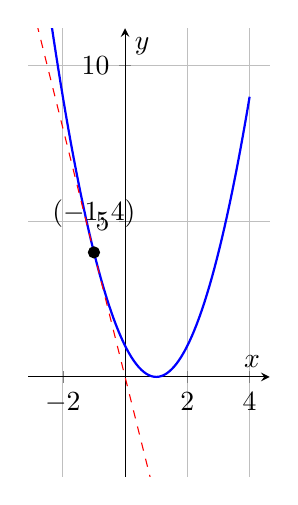
\begin{tikzpicture}
        \begin{axis}[
            axis lines = middle,
            xlabel = $x$,
            ylabel = $y$,
            grid = major,
            samples = 100,
            enlargelimits = true,
            domain = -4:4,
            ymin = -2, ymax = 10, % Ajustar el rango en y
            axis equal image, % Mantiene la proporcionalidad entre ejes
        ]
            % Graficar la parábola
            \addplot[blue, thick] {x^2 - 2*x + 1};
    
            % Graficar la recta tangente en (-1,4)
            \addplot[red, dashed] {(-4)*(x + 1) + 4};
    
            % Punto (-1, 4)
            \addplot[only marks, mark=*, black] coordinates {(-1,4)};
            \node at (axis cs:-1,4.5) [anchor=south] {$(-1, 4)$};
        \end{axis}
    \end{tikzpicture}
\end{center}

La derivada es:
\[
f'(x)=2x-2.
\]
En \( x=-1 \):
\[
f'(-1)=2(-1)-2=-4.
\]
La ecuación de la tangente es:
\begin{align*}
y-4 &= -4\bigl(x-(-1)\bigr)\\
y-4 &= -4(x+1)\\
y &= -4x-4+4\\
y &= -4x.
\end{align*}
\end{solution}

\bigskip

\begin{problem}
Encuentra la ecuación de la recta tangente a la curva \( y = 2x^2 + 1 \) que sea paralela a la recta \( 8x + y - 2 = 0 \).
\end{problem}

\begin{solution}
Calcular la pendiente para \( 8x + y - 2 = 0 \):
\[
    y = -8x + 2
\]
La pendiente, entonces, es \( -8 \) . \\

Igualamos la derivada de la curva a la pendiente para encontrar el punto de tangencia:

\begin{align*}
    4x &= - 8 \\
    x &= - 2
\end{align*}

Por lo tanto, el punto de tangencia es en \( x = -2 \), obteniendo que:

\begin{align*}
    y &= 2*(-2)^2+1 \\
    y &= 9
\end{align*}

El punto de tangencia se da en \( x_0=-2, y_0=9\), por lo que ahora buscamos la ecuación con la pendiente obtenieda previamente y en el punto de tangencia:

\begin{align*}
    y - 9 &= -8(x-(-2)) \\
    y - 9 &= -8(x+2) \\
    y - 9 &= -8x - 16 \\
    y &= -8x - 16 + 9 \\
    y &= -8x - 7
\end{align*}
\end{solution}

\bigskip

\begin{problem}
Encuentra las ecuaciones de las dos rectas que pasan por el punto \((3,1)\) y que son tangentes a la curva \( y = x^2 - 4 \).
\end{problem}

\begin{solution}
Calcular la derivada de \( x^2 - 4 \) asumiendo que \( x= a \):

\[
    f'(a) = 2a
\]
    
Para calcular los puntos de tangencia, en principio, consideramos la ecuación de la pendiente y calculamos los puntos para la parábola \( x^2 - 4 \) y el punto \( (3, 1) \): 

\[
    m = \frac{y_2-y_1}{x_2-x_1}
\]

\begin{align*}
    m &= \frac{a^2-4-1}{a-3} \\
    &= \frac{a^2-5}{a-3}
\end{align*}

Siendo \( m = 2a \):

\begin{align*}
    2a &= \frac{a^2-5}{a-3} \\
    2a(a-3) &= a^2 - 5 \\
    2a^2-6a-a^2+5 &= 0 \\
    a^2-6a+5 &= 0 
\end{align*}

Obtenemos dos valores para \( a \): \( a=5, a=1\). Con ellos, podemos estabelcer las coordenadas de los puntos de tangencia respecto a la párbola:

\begin{align*}
    5^2 - 4 &= 21 \\
    1^2 - 4 &= - 3
\end{align*}

Nuestros puntos de tangencia son: \( (5, 21), (1, -3)\). Ahora podemos calcular las pendientes para cada punto:

\begin{align*}
    m &= \frac{21-1}{5-3} \\
    &= \frac{20}{2} \\
    &= 10
\end{align*}
\begin{align*}
    m &= \frac{-3-1}{1-3} \\
    &= \frac{-4}{-2} \\
    &= 2
\end{align*}

Finalmente, reemplazamos en la ecuación para dar con las dos rectas.

\begin{align*}
    y - 1 &= 10(x-3) \\
    y - 1 &= 10x - 30 \\
    y &= 10x - 30 + 1 \\
    y &= 10x - 29
\end{align*}
\begin{align*}
    y - 1 &= 2(x-3) \\
    y - 1 &= 2x - 6 \\
    y &= 2x - 6 + 1 \\
    y &= 2x - 5
\end{align*}
\end{solution}

\bigskip

\begin{problem}
Demuestra analíticamente que no existe ninguna recta que pase por el punto \((1,-2)\) y sea tangente a la curva \( y = x^2 - 4 \).
\end{problem}

\begin{solution}
Para que una recta sea tangente a \( y=x^2-4 \) debe tocar  la parábola en un único punto \( (a, a^2-4) \) y tener la misma pendiente que la derivada en \( x=a \). \\

Nuestra ecuación quedaría del siguiente modo:

\[
y - (a^2-4) = 2a(x-a)
\]

Ponemos \( 2a \) en tanto resulta la derivada de la parábola y es la pendiente de la recta tangente en cualquier punto.

Ahora, debemos reemplazar el punto dado en la ecuación.

\begin{align*}
    -2 - (a^2-4) &= 2a(1-a) \\
    -2 - a^2 + 4 &= 2a - 2a^2 \\
    -2 - a^2 + 4 - 2a - 2a^2 &= 0 \\
    a^2 - 2a + 2 &= 0
\end{align*}

Dado que las soluciones \( a' = 1 + i \) y \( a'' = 1 - i \) son números complejos, no existen valores reales de \( a \). \\

Por lo tanto, \textbf{no hay ninguna recta real que sea tangente a la parábola y pase por el punto \( (1, -2) \)}.
\end{solution}

\bigskip

\begin{problem}
Una de las rectas que pasa por el punto \((2,0)\) y es tangente a la parábola \( y = x^2 \) es el eje \( x \). Encuentra la ecuación de la otra recta.
\end{problem}

\begin{solution}
Calculamos  el restante punto de tangencia considerando:

\begin{itemize}
    \item \( f'(x) = 2x \)
    \item \( y_0=a^2, x_0=a\)
    \item el punto de interés \( (2, 0) \)
\end{itemize}

\begin{align*}
    2a &= \frac{a^2-0}{a-2} \\
    2a(a-2) &= a^2 \\
    2a^2 - 4a - a^2 &= 0 \\
    a^2 - 4a &= 0
\end{align*}

Esto nos arroja dos valores: \( a' = 0 \) y \( a'' = 4 \). 

De modo que el punto de tangencia que nos faltaba considerar es \( (4, 16) \) ya que \( 4^2 = 16 \). \\

Calculamos la pendiente para ese punto de tangencia respecto del punto de interés:

\begin{align*}
    m &= \frac{16-0}{4-2} \\
    &= 8
\end{align*}

Calculamos la recta que pasa por el punto de interés con la pendiente correspondiente:

\begin{align*}
    y - 0 &= 8(x-2) \\
    y &= 8x - 16
\end{align*}
\end{solution}

\bigskip

\begin{problem}
Encuentra las ecuaciones de las dos rectas que pasan por el punto \((3,13)\) y que son tangentes a la parábola \( y = 6x - x^2 \).
\end{problem}

\begin{solution}

Derivamos la función:

\[
f'(x) = -2x+6
\]

Igualamos la derivada como pendiente de la recta dada por la función y el punto de interés:

\begin{align*}
    -2a+6 &= \frac{-a^2+6a-13}{a-3} \\
    (-2a+6)(a-3) &= -a^2+6a-13 \\
    -2a^2 + 6a + 6a - 18 + a^2 - 6a + 13 &= 0 \\
    -a^2 + 6a - 5 &= 0
\end{align*}

Los puntos de tangencia, para \(a'=5\) y \(a''=1\) son \( (5, 5) \) y \( (1, 5) \), ya que:

\begin{align*}
    -(5^2)+6*5 &= 5 \\
    -(1^2)+6*1 &= 5
\end{align*}

Calculamos la pendiente para cada punto obtenido y el punto de interés:

\begin{align*}
    m &= \frac{13-5}{3-5} \\
    m &= -4
\end{align*}
\begin{align*}
    m &= \frac{13-5}{3-1} \\
    m &= 4
\end{align*}

Obtenemos las dos rectas:

\begin{align*}
    y - 13 &= -4(x-3) \\
    y &= -4x + 12 + 13 \\
    y &= -4x + 25
\end{align*}
\begin{align*}
    y - 13 &= 4(x-3) \\
    y &= 4x - 12 + 13 \\
    y &= 4x + 1
\end{align*}
\end{solution}

\bigskip

\begin{problem}
Dibuja el gráfico de \( y = f(x) = |x - 1| \).
\begin{enumerate}
    \item ¿Hay algún punto en el gráfico en el que no exista recta tangente?
    \item Encuentra \( f'(x_0) \) si \( x_0 > 1 \).  Si \( x_0 < 1 \), ¿qué se puede decir sobre \( f'(x_0) \) y sobre \( x_0 = 1 \)?
\end{enumerate}
\end{problem}

\begin{solution} 
Graficamos:

\begin{center}
    \begin{tikzpicture}
        \begin{axis}[
            axis lines=middle,
            xlabel={$x$},
            ylabel={$y$},
            enlargelimits=true,
            xtick={-2,-1,0,1,2,3,4},
            ytick={0,1,2,3,4},
            domain=-2:4,
            samples=100,
            legend pos=north west
        ]
            \addplot[blue, thick] {abs(x-1)};
        \end{axis}
    \end{tikzpicture}
\end{center}
    
La función \( f(x) = |x - 1| \) se define a trozos:
\[
f(x)=
\begin{cases}
x-1, & x\geq 1,\\
-(x-1), & x<1.
\end{cases}
\]
Por lo tanto:
\begin{itemize}
    \item Para \( x > 1 \), \( f(x)=x-1 \) y \( f'(x)=1 \).
    \item Para \( x < 1 \), \( f(x)=-(x-1)=-x+1 \) y \( f'(x)=-1 \).
\end{itemize}
En \( x = 1 \) se tiene:
\[
\lim_{x\to1^+} f'(x)=1 \quad\text{y}\quad \lim_{x\to1^-} f'(x)=-1,
\]
por lo que la derivada no existe en \( x = 1 \). Este es un punto de no diferenciabilidad (cúspide).
\end{solution}

\end{document}
